% Bootstrap Capability: Prompt-Managed Workflow Engineering
% Slide Deck Presentation
\documentclass[aspectratio=169]{beamer}

% Theme and Colors
\usetheme{Madrid}
\usecolortheme{seahorse}
\setbeamertemplate{navigation symbols}{}
\setbeamertemplate{footline}[frame number]

% Packages
\usepackage[utf8]{inputenc}
\usepackage{amsmath,amssymb}
\usepackage{listings}
\usepackage{xcolor}
\usepackage{booktabs}
\usepackage{graphicx}
\usepackage{tikz}
\usepackage{pifont}
\usepackage{marvosym}

\usetikzlibrary{shapes.geometric, shapes.symbols, arrows.meta, positioning, fit, backgrounds, calc, shadows, decorations.pathreplacing}

% Icon replacements (no fontawesome5 needed)
\newcommand{\faCheck}{\ding{51}}
\newcommand{\faTimes}{\ding{55}}
\newcommand{\faEye}{$\odot$}
\newcommand{\faPlay}{$\triangleright$}
\newcommand{\faExclamationTriangle}{$\triangle$!}
\newcommand{\faLightbulb}{$\star$}
\newcommand{\faUser}{$\circ$}
\newcommand{\faLaptopCode}{$\square$}
\newcommand{\faServer}{$\boxplus$}
\newcommand{\faCloud}{$\Diamond$}
\newcommand{\faEnvelope}{\Letter}

% Custom Colors
\definecolor{noaablue}{RGB}{0, 51, 102}
\definecolor{dryrungreen}{RGB}{46, 139, 87}
\definecolor{supervisedorange}{RGB}{230, 126, 34}
\definecolor{sideeffectred}{RGB}{192, 57, 43}
\definecolor{readonlyblue}{RGB}{52, 152, 219}

% Beamer color customization
\setbeamercolor{title}{fg=noaablue}
\setbeamercolor{frametitle}{fg=noaablue}
\setbeamercolor{structure}{fg=noaablue}

% Code listing setup
\lstset{
    basicstyle=\ttfamily\scriptsize,
    breaklines=true,
    frame=single,
    backgroundcolor=\color{gray!10},
    keywordstyle=\color{blue},
    commentstyle=\color{green!60!black},
    stringstyle=\color{red}
}

% Title Information
\title{\textbf{Bootstrap Capability}}
\subtitle{Prompt-Managed Workflow Engineering}
\author{NOAA EMC Global Workflow MCP Team}
\institute{Environmental Modeling Center\\National Oceanic and Atmospheric Administration}
\date{January 6, 2026}

\begin{document}

%------------------------------------------------------------------------------
% Title Slide
%------------------------------------------------------------------------------
\begin{frame}
\titlepage
\end{frame}

%------------------------------------------------------------------------------
% Agenda
%------------------------------------------------------------------------------
\begin{frame}{Agenda}
\begin{columns}[T]
\begin{column}{0.5\textwidth}
\tableofcontents[sections={1-4}]
\end{column}
\begin{column}{0.5\textwidth}
\tableofcontents[sections={5-8}]
\end{column}
\end{columns}
\end{frame}

\section{The Problem}

%------------------------------------------------------------------------------
% The Problem
%------------------------------------------------------------------------------
\begin{frame}{The Problem: AI Code Generation Gap}
\begin{columns}[T]
\begin{column}{0.55\textwidth}
\begin{block}{Current Challenges}
\begin{itemize}
    \item AI generates code without \textbf{execution plan visibility}
    \item No preview of what will change before it changes
    \item Difficult to audit or roll back autonomous actions
    \item Human oversight requires manual intervention
\end{itemize}
\end{block}

\vspace{0.5em}

\begin{alertblock}{The Gap}
Natural language intent $\rightarrow$ ??? $\rightarrow$ Executable code
\end{alertblock}
\end{column}

\begin{column}{0.42\textwidth}
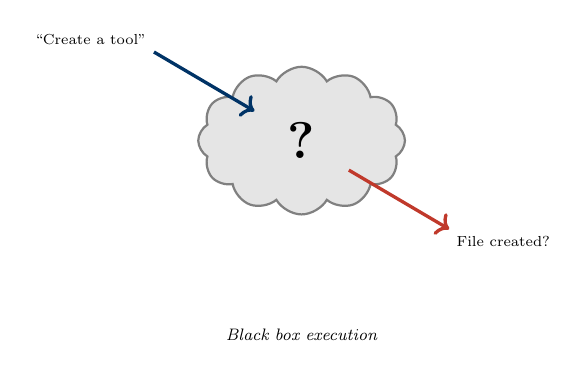
\begin{tikzpicture}[scale=0.75, transform shape]
    % Question mark cloud
    \node[cloud, cloud puffs=12, cloud puff arc=120, 
          minimum width=3.5cm, minimum height=2.5cm,
          draw=gray, fill=gray!20, thick] (cloud) {};
    \node at (cloud) {\Huge\textbf{?}};
    
    % Input arrow
    \draw[->, very thick, noaablue] (-2.5, 1.5) -- (-0.8, 0.5);
    \node[above left, font=\scriptsize] at (-2.5, 1.5) {``Create a tool''};
    
    % Output arrow
    \draw[->, very thick, sideeffectred] (0.8, -0.5) -- (2.5, -1.5);
    \node[below right, font=\scriptsize] at (2.5, -1.5) {File created?};
    
    % Labels
    \node[below=1.8cm of cloud, font=\footnotesize\itshape, text width=3cm, align=center] 
        {Black box execution};
\end{tikzpicture}
\end{column}
\end{columns}
\end{frame}

\section{The Solution}

%------------------------------------------------------------------------------
% The Solution Overview
%------------------------------------------------------------------------------
\begin{frame}{The Solution: Spec-Driven Development (SDD)}
\begin{center}
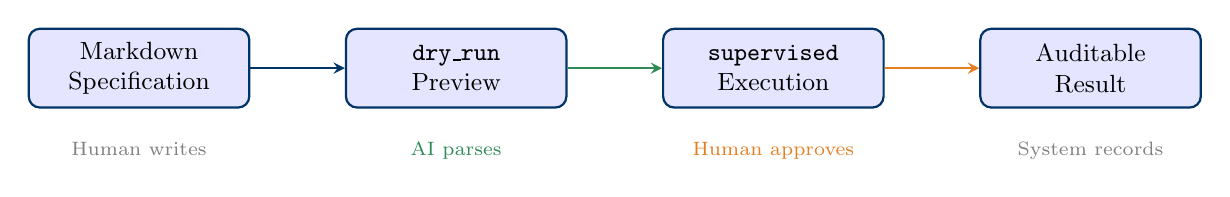
\begin{tikzpicture}[
    node distance=1.2cm,
    box/.style={rectangle, rounded corners, draw=noaablue, fill=blue!10, 
                thick, minimum width=2.8cm, minimum height=1cm, align=center, font=\small},
    arrow/.style={->, thick, >=stealth}
]
    % Boxes
    \node[box] (spec) {Markdown\\Specification};
    \node[box, right=of spec] (dryrun) {\texttt{dry\_run}\\Preview};
    \node[box, right=of dryrun] (supervised) {\texttt{supervised}\\Execution};
    \node[box, right=of supervised] (result) {Auditable\\Result};
    
    % Arrows
    \draw[arrow, noaablue] (spec) -- (dryrun);
    \draw[arrow, dryrungreen] (dryrun) -- (supervised);
    \draw[arrow, supervisedorange] (supervised) -- (result);
    
    % Labels below
    \node[below=0.3cm of spec, font=\scriptsize, text=gray] {Human writes};
    \node[below=0.3cm of dryrun, font=\scriptsize, text=dryrungreen] {AI parses};
    \node[below=0.3cm of supervised, font=\scriptsize, text=supervisedorange] {Human approves};
    \node[below=0.3cm of result, font=\scriptsize, text=gray] {System records};
\end{tikzpicture}
\end{center}

\vspace{0.5em}

\begin{columns}[T]
\begin{column}{0.48\textwidth}
\begin{block}{Key Principle}
\centering
\textbf{``If it's not in the SDD, it doesn't get coded.''}
\end{block}
\end{column}
\begin{column}{0.48\textwidth}
\begin{block}{Benefit}
\centering
Full visibility + Human control + Audit trail
\end{block}
\end{column}
\end{columns}
\end{frame}

\section{Execution Model}

%------------------------------------------------------------------------------
% The Two Modes - Visual
%------------------------------------------------------------------------------
\begin{frame}{Two Execution Modes}
\begin{center}
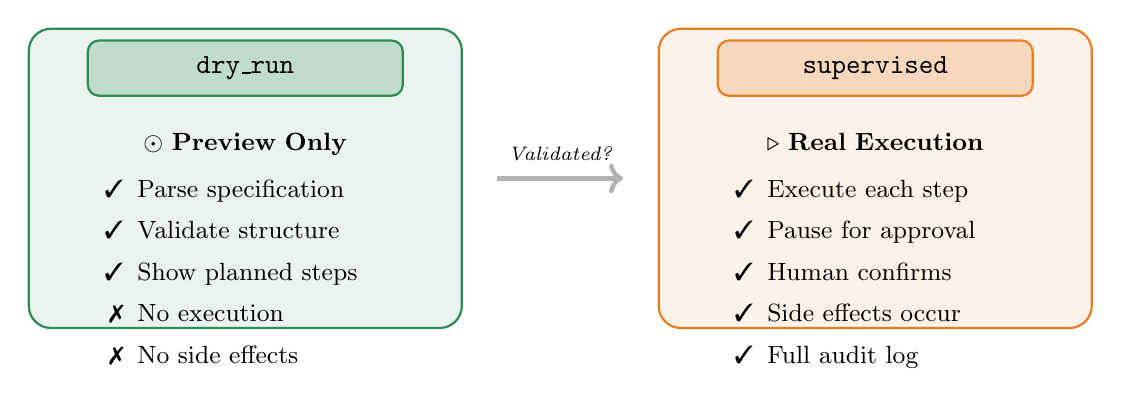
\begin{tikzpicture}[
    node distance=0.8cm,
    modebox/.style={rectangle, rounded corners=8pt, thick, 
                    minimum width=5.5cm, minimum height=3.8cm, align=center},
    titlebox/.style={rectangle, rounded corners=4pt, thick, 
                     minimum width=4cm, minimum height=0.7cm, font=\bfseries}
]
    % dry_run box
    \node[modebox, draw=dryrungreen, fill=dryrungreen!10] (drybox) at (-4, 0) {};
    \node[titlebox, draw=dryrungreen, fill=dryrungreen!30] at (-4, 1.4) {\texttt{dry\_run}};
    
    \node[below=0.1cm, font=\small, text width=4.5cm, align=center] at (-4, 0.8) {
        \faEye\ \textbf{Preview Only}\\[0.5em]
        \begin{itemize}
            \item[\faCheck] Parse specification
            \item[\faCheck] Validate structure
            \item[\faCheck] Show planned steps
            \item[\faTimes] No execution
            \item[\faTimes] No side effects
        \end{itemize}
    };
    
    % supervised box
    \node[modebox, draw=supervisedorange, fill=supervisedorange!10] (supbox) at (4, 0) {};
    \node[titlebox, draw=supervisedorange, fill=supervisedorange!30] at (4, 1.4) {\texttt{supervised}};
    
    \node[below=0.1cm, font=\small, text width=4.5cm, align=center] at (4, 0.8) {
        \faPlay\ \textbf{Real Execution}\\[0.5em]
        \begin{itemize}
            \item[\faCheck] Execute each step
            \item[\faCheck] Pause for approval
            \item[\faCheck] Human confirms
            \item[\faCheck] Side effects occur
            \item[\faCheck] Full audit log
        \end{itemize}
    };
    
    % Arrow between
    \draw[->, ultra thick, gray!60] (-0.8, 0) -- (0.8, 0);
    \node[above=0.1cm, font=\scriptsize\itshape] at (0, 0) {Validated?};
\end{tikzpicture}
\end{center}
\end{frame}

%------------------------------------------------------------------------------
% Key Insight
%------------------------------------------------------------------------------
\begin{frame}{Key Insight}
\begin{center}
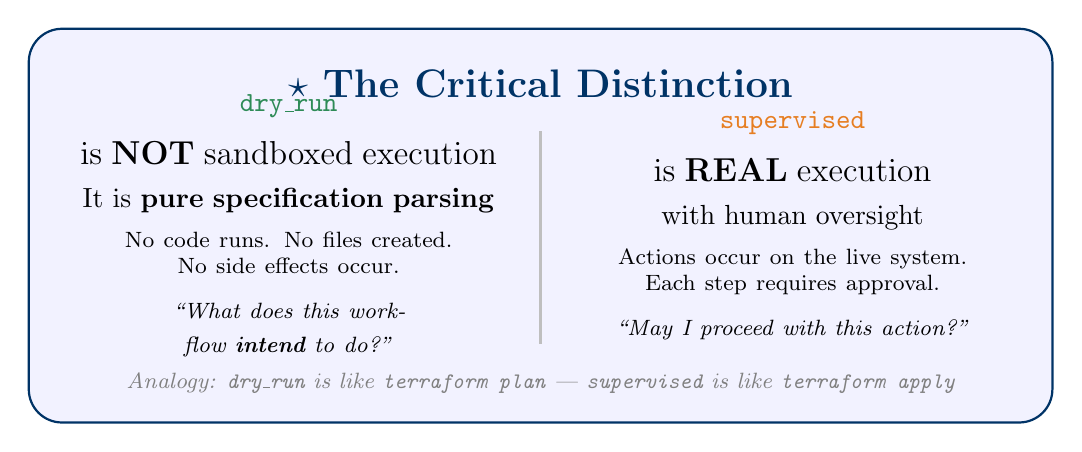
\begin{tikzpicture}
    % Background box
    \node[rectangle, rounded corners=12pt, draw=noaablue, fill=blue!5, 
          thick, minimum width=13cm, minimum height=5cm] (insight) {};
    
    % Title
    \node[font=\Large\bfseries, text=noaablue] at (0, 1.8) 
        {\faLightbulb\ The Critical Distinction};
    
    % Two columns
    \node[text width=5.5cm, align=center] at (-3.2, 0) {
        \textcolor{dryrungreen}{\texttt{\textbf{dry\_run}}}\\[0.5em]
        \large is \textbf{NOT} sandboxed execution\\[0.3em]
        \normalsize It is \textbf{pure specification parsing}\\[0.5em]
        \footnotesize No code runs. No files created.\\
        No side effects occur.\\[0.5em]
        \textit{``What does this workflow \textbf{intend} to do?''}
    };
    
    \draw[thick, gray!50] (0, -1.5) -- (0, 1.2);
    
    \node[text width=5.5cm, align=center] at (3.2, 0) {
        \textcolor{supervisedorange}{\texttt{\textbf{supervised}}}\\[0.5em]
        \large is \textbf{REAL} execution\\[0.3em]
        \normalsize with human oversight\\[0.5em]
        \footnotesize Actions occur on the live system.\\
        Each step requires approval.\\[0.5em]
        \textit{``May I proceed with this action?''}
    };
    
    % Analogy
    \node[font=\footnotesize\itshape, text=gray] at (0, -2) 
        {Analogy: \texttt{dry\_run} is like \texttt{terraform plan} — 
         \texttt{supervised} is like \texttt{terraform apply}};
\end{tikzpicture}
\end{center}
\end{frame}

\section{Side-Effect Classification}

%------------------------------------------------------------------------------
% Side Effect Classification
%------------------------------------------------------------------------------
\begin{frame}{Side-Effect Classification}
\begin{columns}[T]
\begin{column}{0.48\textwidth}
\begin{block}{\textcolor{readonlyblue}{\faEye\ Read-Only Steps}}
\textbf{Auto-execute} — No approval needed
\vspace{0.3em}
\begin{itemize}
    \item \texttt{health\_check}
    \item \texttt{validation}
    \item \texttt{data\_query}
    \item \texttt{analysis}
\end{itemize}
\vspace{0.3em}
\footnotesize\textit{These steps only observe; they cannot modify state.}
\end{block}
\end{column}

\begin{column}{0.48\textwidth}
\begin{alertblock}{\textcolor{sideeffectred}{\faExclamationTriangle\ Side-Effect Steps}}
\textbf{Require approval} — Human must confirm
\vspace{0.3em}
\begin{itemize}
    \item \texttt{code\_generation}
    \item \texttt{code\_modification}
    \item \texttt{command}
    \item \texttt{ingestion}
    \item \texttt{file\_delete}
    \item \texttt{git\_operation}
\end{itemize}
\end{alertblock}
\end{column}
\end{columns}

\vspace{0.5em}
\begin{center}
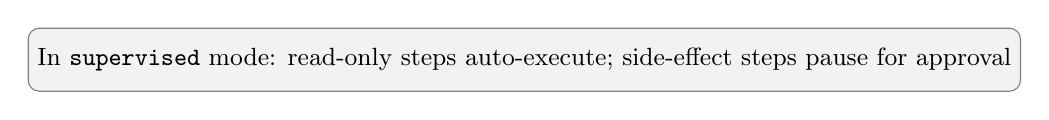
\begin{tikzpicture}
    \node[rectangle, rounded corners, draw=gray, fill=gray!10, 
          minimum width=11cm, minimum height=0.8cm, font=\small] {
        In \texttt{supervised} mode: read-only steps auto-execute; 
        side-effect steps pause for approval
    };
\end{tikzpicture}
\end{center}
\end{frame}

\section{The Iterative Loop}

%------------------------------------------------------------------------------
% Iterative Development Loop - Full Diagram
%------------------------------------------------------------------------------
\begin{frame}{The Iterative Development Loop}
\begin{center}
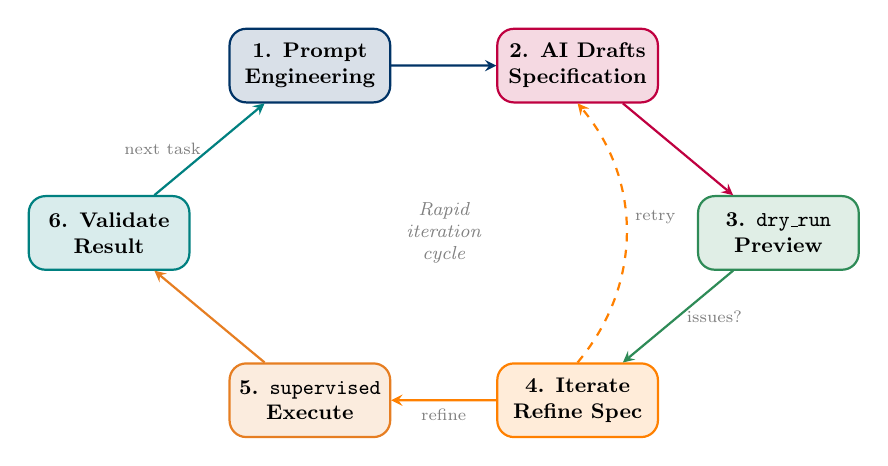
\begin{tikzpicture}[
    scale=0.85, transform shape,
    node distance=1.5cm,
    phase/.style={rectangle, rounded corners=6pt, draw=#1, fill=#1!15, 
                  thick, minimum width=2.4cm, minimum height=1.1cm, 
                  align=center, font=\small\bfseries},
    arrow/.style={->, thick, >=stealth},
    label/.style={font=\scriptsize, text=gray}
]
    % Phases in a cycle
    \node[phase=noaablue] (prompt) at (0, 2.5) {1. Prompt\\Engineering};
    \node[phase=purple] (draft) at (4, 2.5) {2. AI Drafts\\Specification};
    \node[phase=dryrungreen] (dryrun) at (7, 0) {3. \texttt{dry\_run}\\Preview};
    \node[phase=orange] (iterate) at (4, -2.5) {4. Iterate\\Refine Spec};
    \node[phase=supervisedorange] (execute) at (0, -2.5) {5. \texttt{supervised}\\Execute};
    \node[phase=teal] (validate) at (-3, 0) {6. Validate\\Result};
    
    % Main flow arrows
    \draw[arrow, noaablue] (prompt) -- (draft);
    \draw[arrow, purple] (draft) -- (dryrun);
    \draw[arrow, dryrungreen] (dryrun) -- node[right, label] {issues?} (iterate);
    \draw[arrow, orange] (iterate) -- node[below, label] {refine} (execute);
    \draw[arrow, supervisedorange] (execute) -- (validate);
    \draw[arrow, teal] (validate) -- node[left, label] {next task} (prompt);
    
    % Iteration loop back
    \draw[arrow, orange, dashed] (iterate.north) to[bend right=40] 
        node[above right, label] {retry} (draft.south);
    
    % Center label
    \node[font=\footnotesize\itshape, text=gray, align=center] at (2, 0) {
        Rapid\\iteration\\cycle
    };
\end{tikzpicture}
\end{center}
\end{frame}

%------------------------------------------------------------------------------
% Loop Details
%------------------------------------------------------------------------------
\begin{frame}{Loop Phase Details}
\begin{center}
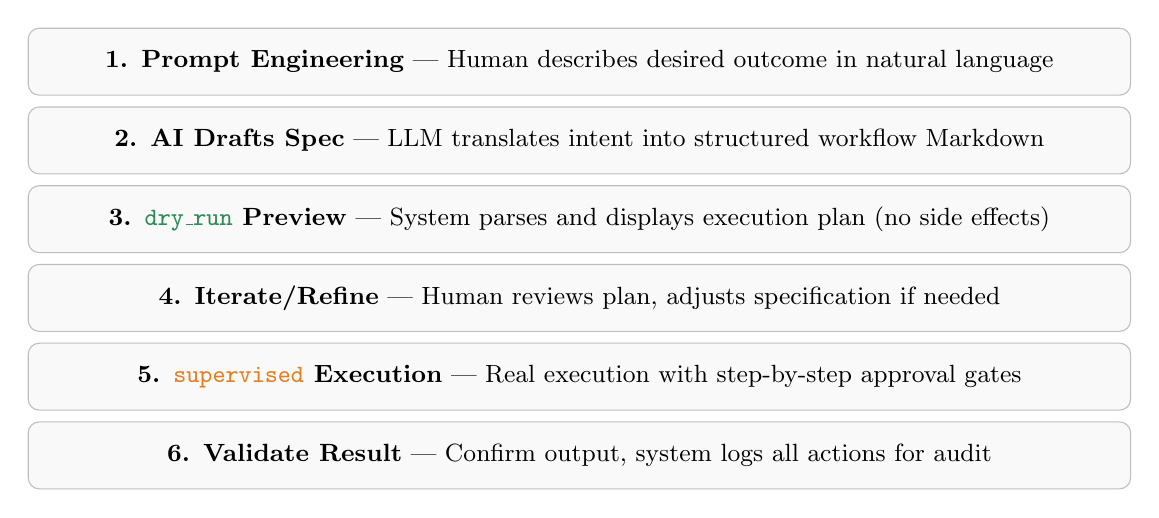
\begin{tikzpicture}[
    node distance=0.3cm,
    phasebox/.style={rectangle, rounded corners=4pt, draw=gray!50, fill=gray!5, 
                     minimum width=14cm, minimum height=0.85cm, font=\small}
]
    \node[phasebox] (p1) at (0, 2.4) {
        \textbf{1. Prompt Engineering} — Human describes desired outcome in natural language
    };
    \node[phasebox] (p2) at (0, 1.4) {
        \textbf{2. AI Drafts Spec} — LLM translates intent into structured workflow Markdown
    };
    \node[phasebox] (p3) at (0, 0.4) {
        \textbf{3. \textcolor{dryrungreen}{\texttt{dry\_run}} Preview} — System parses and displays execution plan (no side effects)
    };
    \node[phasebox] (p4) at (0, -0.6) {
        \textbf{4. Iterate/Refine} — Human reviews plan, adjusts specification if needed
    };
    \node[phasebox] (p5) at (0, -1.6) {
        \textbf{5. \textcolor{supervisedorange}{\texttt{supervised}} Execution} — Real execution with step-by-step approval gates
    };
    \node[phasebox] (p6) at (0, -2.6) {
        \textbf{6. Validate Result} — Confirm output, system logs all actions for audit
    };
\end{tikzpicture}
\end{center}

\vspace{0.3em}
\begin{block}{Why This Works}
\begin{itemize}
    \item \textbf{Fast feedback}: \texttt{dry\_run} is instantaneous — iterate without risk
    \item \textbf{Human in the loop}: Every side effect requires explicit approval
    \item \textbf{Full auditability}: Complete record of what was planned vs. executed
\end{itemize}
\end{block}
\end{frame}

\section{Workflow Format}

%------------------------------------------------------------------------------
% Workflow Specification Format
%------------------------------------------------------------------------------
\begin{frame}[fragile]{Workflow Specification Format}
\begin{columns}[T]
\begin{column}{0.52\textwidth}
\begin{block}{Step Definition Structure}
\begin{lstlisting}
### Step 3: Generate Example Tool
**Type**: code_generation
**Target**: src/tools/ExampleTool.js
**Template**: basic-mcp-tool
**Required**: Yes
**Variables**:
- className: ExampleTool
- toolName: example_operation
- description: Example tool
\end{lstlisting}
\end{block}
\end{column}

\begin{column}{0.45\textwidth}
\begin{block}{Key Fields}
\begin{description}
    \item[Type] Step category (determines approval)
    \item[Target] File or resource affected
    \item[Template] Code template to use
    \item[Required] Can workflow continue if this fails?
    \item[Variables] Parameters for interpolation
\end{description}
\end{block}
\end{column}
\end{columns}

\vspace{0.3em}
\begin{center}
\footnotesize\textit{Workflows are just Markdown files — version controlled, diffable, reviewable}
\end{center}
\end{frame}

%------------------------------------------------------------------------------
% Template System
%------------------------------------------------------------------------------
\begin{frame}[fragile]{Template Interpolation System}
\begin{columns}[T]
\begin{column}{0.48\textwidth}
\begin{block}{Template (basic-mcp-tool.template)}
\begin{lstlisting}
class {{className}} {
  constructor() {
    this.name = '{{toolName}}';
    this.description = 
      '{{description}}';
  }
  
  async execute(params) {
    // Implementation
    return { success: true };
  }
}

module.exports = { {{className}} };
\end{lstlisting}
\end{block}
\end{column}

\begin{column}{0.48\textwidth}
\begin{block}{Generated Output}
\begin{lstlisting}
class ExampleTool {
  constructor() {
    this.name = 'example_operation';
    this.description = 
      'Example tool';
  }
  
  async execute(params) {
    // Implementation
    return { success: true };
  }
}

module.exports = { ExampleTool };
\end{lstlisting}
\end{block}
\end{column}
\end{columns}

\vspace{0.3em}
\begin{center}
\texttt{\{\{variableName\}\}} $\rightarrow$ replaced with workflow-specified values
\end{center}
\end{frame}

\section{Bootstrap Demo}

%------------------------------------------------------------------------------
% Bootstrap Demo Architecture
%------------------------------------------------------------------------------
\begin{frame}{Bootstrap Capability Demo}
\begin{center}
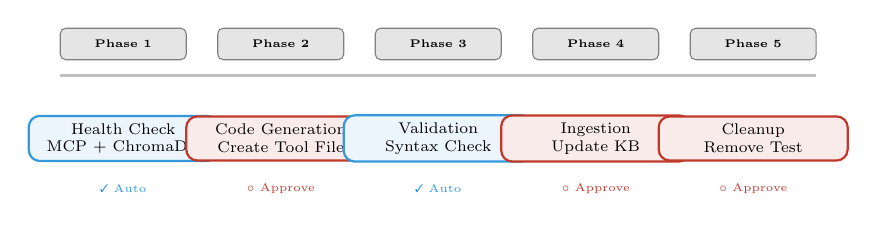
\begin{tikzpicture}[
    scale=0.8, transform shape,
    node distance=0.8cm,
    box/.style={rectangle, rounded corners=4pt, draw=#1, fill=#1!10, 
                thick, minimum width=3cm, minimum height=0.7cm, 
                align=center, font=\scriptsize},
    phase/.style={rectangle, rounded corners=2pt, draw=gray, fill=gray!20, 
                  minimum width=2cm, minimum height=0.5cm, font=\tiny\bfseries}
]
    % Timeline
    \draw[thick, gray!50] (-6, 0) -- (6, 0);
    
    % Phase markers
    \node[phase] at (-5, 0.5) {Phase 1};
    \node[phase] at (-2.5, 0.5) {Phase 2};
    \node[phase] at (0, 0.5) {Phase 3};
    \node[phase] at (2.5, 0.5) {Phase 4};
    \node[phase] at (5, 0.5) {Phase 5};
    
    % Steps
    \node[box=readonlyblue] at (-5, -1) {Health Check\\MCP + ChromaDB};
    \node[box=sideeffectred] at (-2.5, -1) {Code Generation\\Create Tool File};
    \node[box=readonlyblue] at (0, -1) {Validation\\Syntax Check};
    \node[box=sideeffectred] at (2.5, -1) {Ingestion\\Update KB};
    \node[box=sideeffectred] at (5, -1) {Cleanup\\Remove Test};
    
    % Approval indicators
    \node[font=\tiny, text=readonlyblue] at (-5, -1.8) {\faCheck\ Auto};
    \node[font=\tiny, text=sideeffectred] at (-2.5, -1.8) {\faUser\ Approve};
    \node[font=\tiny, text=readonlyblue] at (0, -1.8) {\faCheck\ Auto};
    \node[font=\tiny, text=sideeffectred] at (2.5, -1.8) {\faUser\ Approve};
    \node[font=\tiny, text=sideeffectred] at (5, -1.8) {\faUser\ Approve};
\end{tikzpicture}
\end{center}

\vspace{0.5em}
\begin{columns}[T]
\begin{column}{0.48\textwidth}
\begin{block}{What It Demonstrates}
\begin{itemize}
    \item Full code generation from template
    \item Syntax validation of generated code
    \item Knowledge base integration
    \item Clean teardown
\end{itemize}
\end{block}
\end{column}
\begin{column}{0.48\textwidth}
\begin{block}{Output}
\begin{itemize}
    \item \texttt{ExampleBootstrapTool.js} — 1,888 bytes
    \item Valid JavaScript syntax
    \item MCP tool pattern compliant
    \item Full execution audit log
\end{itemize}
\end{block}
\end{column}
\end{columns}
\end{frame}

\section{Future Work}

%------------------------------------------------------------------------------
% Future Vision
%------------------------------------------------------------------------------
\begin{frame}{Future: Self-Evolving Systems}
\begin{center}
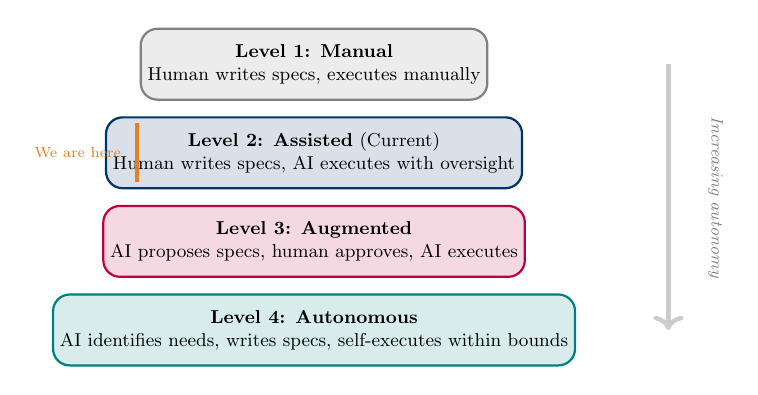
\begin{tikzpicture}[
    scale=0.75, transform shape,
    node distance=1cm,
    level/.style={rectangle, rounded corners=6pt, draw=#1, fill=#1!15, 
                  thick, minimum width=5cm, minimum height=1.2cm, 
                  align=center, font=\small}
]
    % Evolution levels
    \node[level=gray] (l1) at (0, 3) {\textbf{Level 1: Manual}\\Human writes specs, executes manually};
    \node[level=noaablue] (l2) at (0, 1.5) {\textbf{Level 2: Assisted} (Current)\\Human writes specs, AI executes with oversight};
    \node[level=purple] (l3) at (0, 0) {\textbf{Level 3: Augmented}\\AI proposes specs, human approves, AI executes};
    \node[level=teal] (l4) at (0, -1.5) {\textbf{Level 4: Autonomous}\\AI identifies needs, writes specs, self-executes within bounds};
    
    % Arrow
    \draw[->, ultra thick, gray!40] (6, 3) -- (6, -1.5);
    \node[rotate=-90, font=\footnotesize\itshape, text=gray] at (6.8, 0.75) {Increasing autonomy};
    
    % Current marker
    \draw[very thick, supervisedorange] (-3, 1) -- (-3, 2);
    \node[font=\scriptsize, text=supervisedorange] at (-4, 1.5) {We are here};
\end{tikzpicture}
\end{center}

\vspace{0.3em}
\begin{block}{Goal: Controlled Self-Evolution}
Systems that can bootstrap new capabilities while maintaining human oversight and audit trails
\end{block}
\end{frame}

%------------------------------------------------------------------------------
% Deployment Modes
%------------------------------------------------------------------------------
\begin{frame}{Three Deployment Scenarios}
\begin{center}
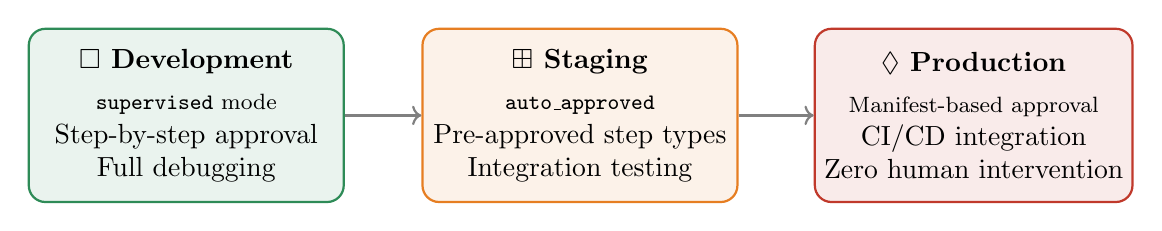
\begin{tikzpicture}[
    node distance=0.5cm,
    scenario/.style={rectangle, rounded corners=6pt, draw=#1, fill=#1!10, 
                     thick, minimum width=4cm, minimum height=2.2cm, align=center}
]
    \node[scenario=dryrungreen] (dev) at (-5, 0) {
        \textbf{\faLaptopCode\ Development}\\[0.3em]
        \footnotesize\texttt{supervised} mode\\
        Step-by-step approval\\
        Full debugging
    };
    
    \node[scenario=supervisedorange] (staging) at (0, 0) {
        \textbf{\faServer\ Staging}\\[0.3em]
        \footnotesize\texttt{auto\_approved}\\
        Pre-approved step types\\
        Integration testing
    };
    
    \node[scenario=sideeffectred] (prod) at (5, 0) {
        \textbf{\faCloud\ Production}\\[0.3em]
        \footnotesize Manifest-based approval\\
        CI/CD integration\\
        Zero human intervention
    };
    
    % Arrows
    \draw[->, thick, gray] (dev) -- (staging);
    \draw[->, thick, gray] (staging) -- (prod);
\end{tikzpicture}
\end{center}

\vspace{0.5em}
\begin{center}
\footnotesize
\textbf{Same workflow specification} → Different execution modes → Appropriate oversight level
\end{center}
\end{frame}

\section{Summary}

%------------------------------------------------------------------------------
% Summary
%------------------------------------------------------------------------------
\begin{frame}{Summary: Bootstrap Capability}
\begin{columns}[T]
\begin{column}{0.55\textwidth}
\begin{block}{What We Built}
\begin{itemize}
    \item \textbf{Spec-Driven Development} — Markdown workflows as source of truth
    \item \textbf{Two-Phase Execution} — \texttt{dry\_run} + \texttt{supervised}
    \item \textbf{Side-Effect Gates} — Human approval for mutations
    \item \textbf{Template System} — Reusable code generation
    \item \textbf{Full Auditability} — Every action logged
\end{itemize}
\end{block}
\end{column}

\begin{column}{0.42\textwidth}
\begin{alertblock}{Key Takeaway}
\centering
\Large
\textbf{Preview} before \textbf{Execute}\\[0.5em]
\normalsize
\texttt{dry\_run} $\rightarrow$ \texttt{supervised}
\end{alertblock}

\vspace{0.5em}

\begin{exampleblock}{Result}
AI-assisted code generation with\\
\textbf{human oversight} and\\
\textbf{complete audit trail}
\end{exampleblock}
\end{column}
\end{columns}
\end{frame}

%------------------------------------------------------------------------------
% Questions
%------------------------------------------------------------------------------
\begin{frame}
\begin{center}
\Huge\textbf{Questions?}

\vspace{2em}

\Large
\faEnvelope\ \texttt{Terry.McGuinness@noaa.gov}

\vspace{1em}

\normalsize
NOAA Environmental Modeling Center\\
Global Workflow MCP Team

\vspace{2em}

\footnotesize
\textit{Source: Bootstrap Capability White Paper, January 2026}
\end{center}
\end{frame}

%------------------------------------------------------------------------------
% Appendix - Comparison Table
%------------------------------------------------------------------------------
\begin{frame}{Appendix: Mode Comparison}
\begin{center}
\begin{tabular}{l|ccc}
\toprule
\textbf{Characteristic} & \texttt{dry\_run} & \texttt{supervised} & \texttt{auto\_approved} \\
\midrule
Parse specification & \textcolor{dryrungreen}{\faCheck} & \textcolor{dryrungreen}{\faCheck} & \textcolor{dryrungreen}{\faCheck} \\
Execute read-only steps & \textcolor{sideeffectred}{\faTimes} & \textcolor{dryrungreen}{\faCheck} & \textcolor{dryrungreen}{\faCheck} \\
Execute side-effect steps & \textcolor{sideeffectred}{\faTimes} & \textcolor{dryrungreen}{\faCheck} & \textcolor{dryrungreen}{\faCheck} \\
Human approval gates & N/A & \textcolor{dryrungreen}{\faCheck} & \textcolor{sideeffectred}{\faTimes} \\
Files/state modified & \textcolor{sideeffectred}{\faTimes} & \textcolor{dryrungreen}{\faCheck} & \textcolor{dryrungreen}{\faCheck} \\
Suitable for CI/CD & \textcolor{sideeffectred}{\faTimes} & \textcolor{sideeffectred}{\faTimes} & \textcolor{dryrungreen}{\faCheck} \\
\bottomrule
\end{tabular}
\end{center}

\vspace{1em}

\begin{center}
\footnotesize
\textcolor{dryrungreen}{\faCheck} = Yes \quad 
\textcolor{sideeffectred}{\faTimes} = No \quad
N/A = Not applicable
\end{center}
\end{frame}

\end{document}
